%----------------------------------------------------------------------------------------
%	SLIDE 5.
%----------------------------------------------------------------------------------------
\begin{frame}
\frametitle{Approximations of the Kepler frequency}

\begin{columns}
\begin{column}{0.5\textwidth}
	\begin{figure}
		\centering
		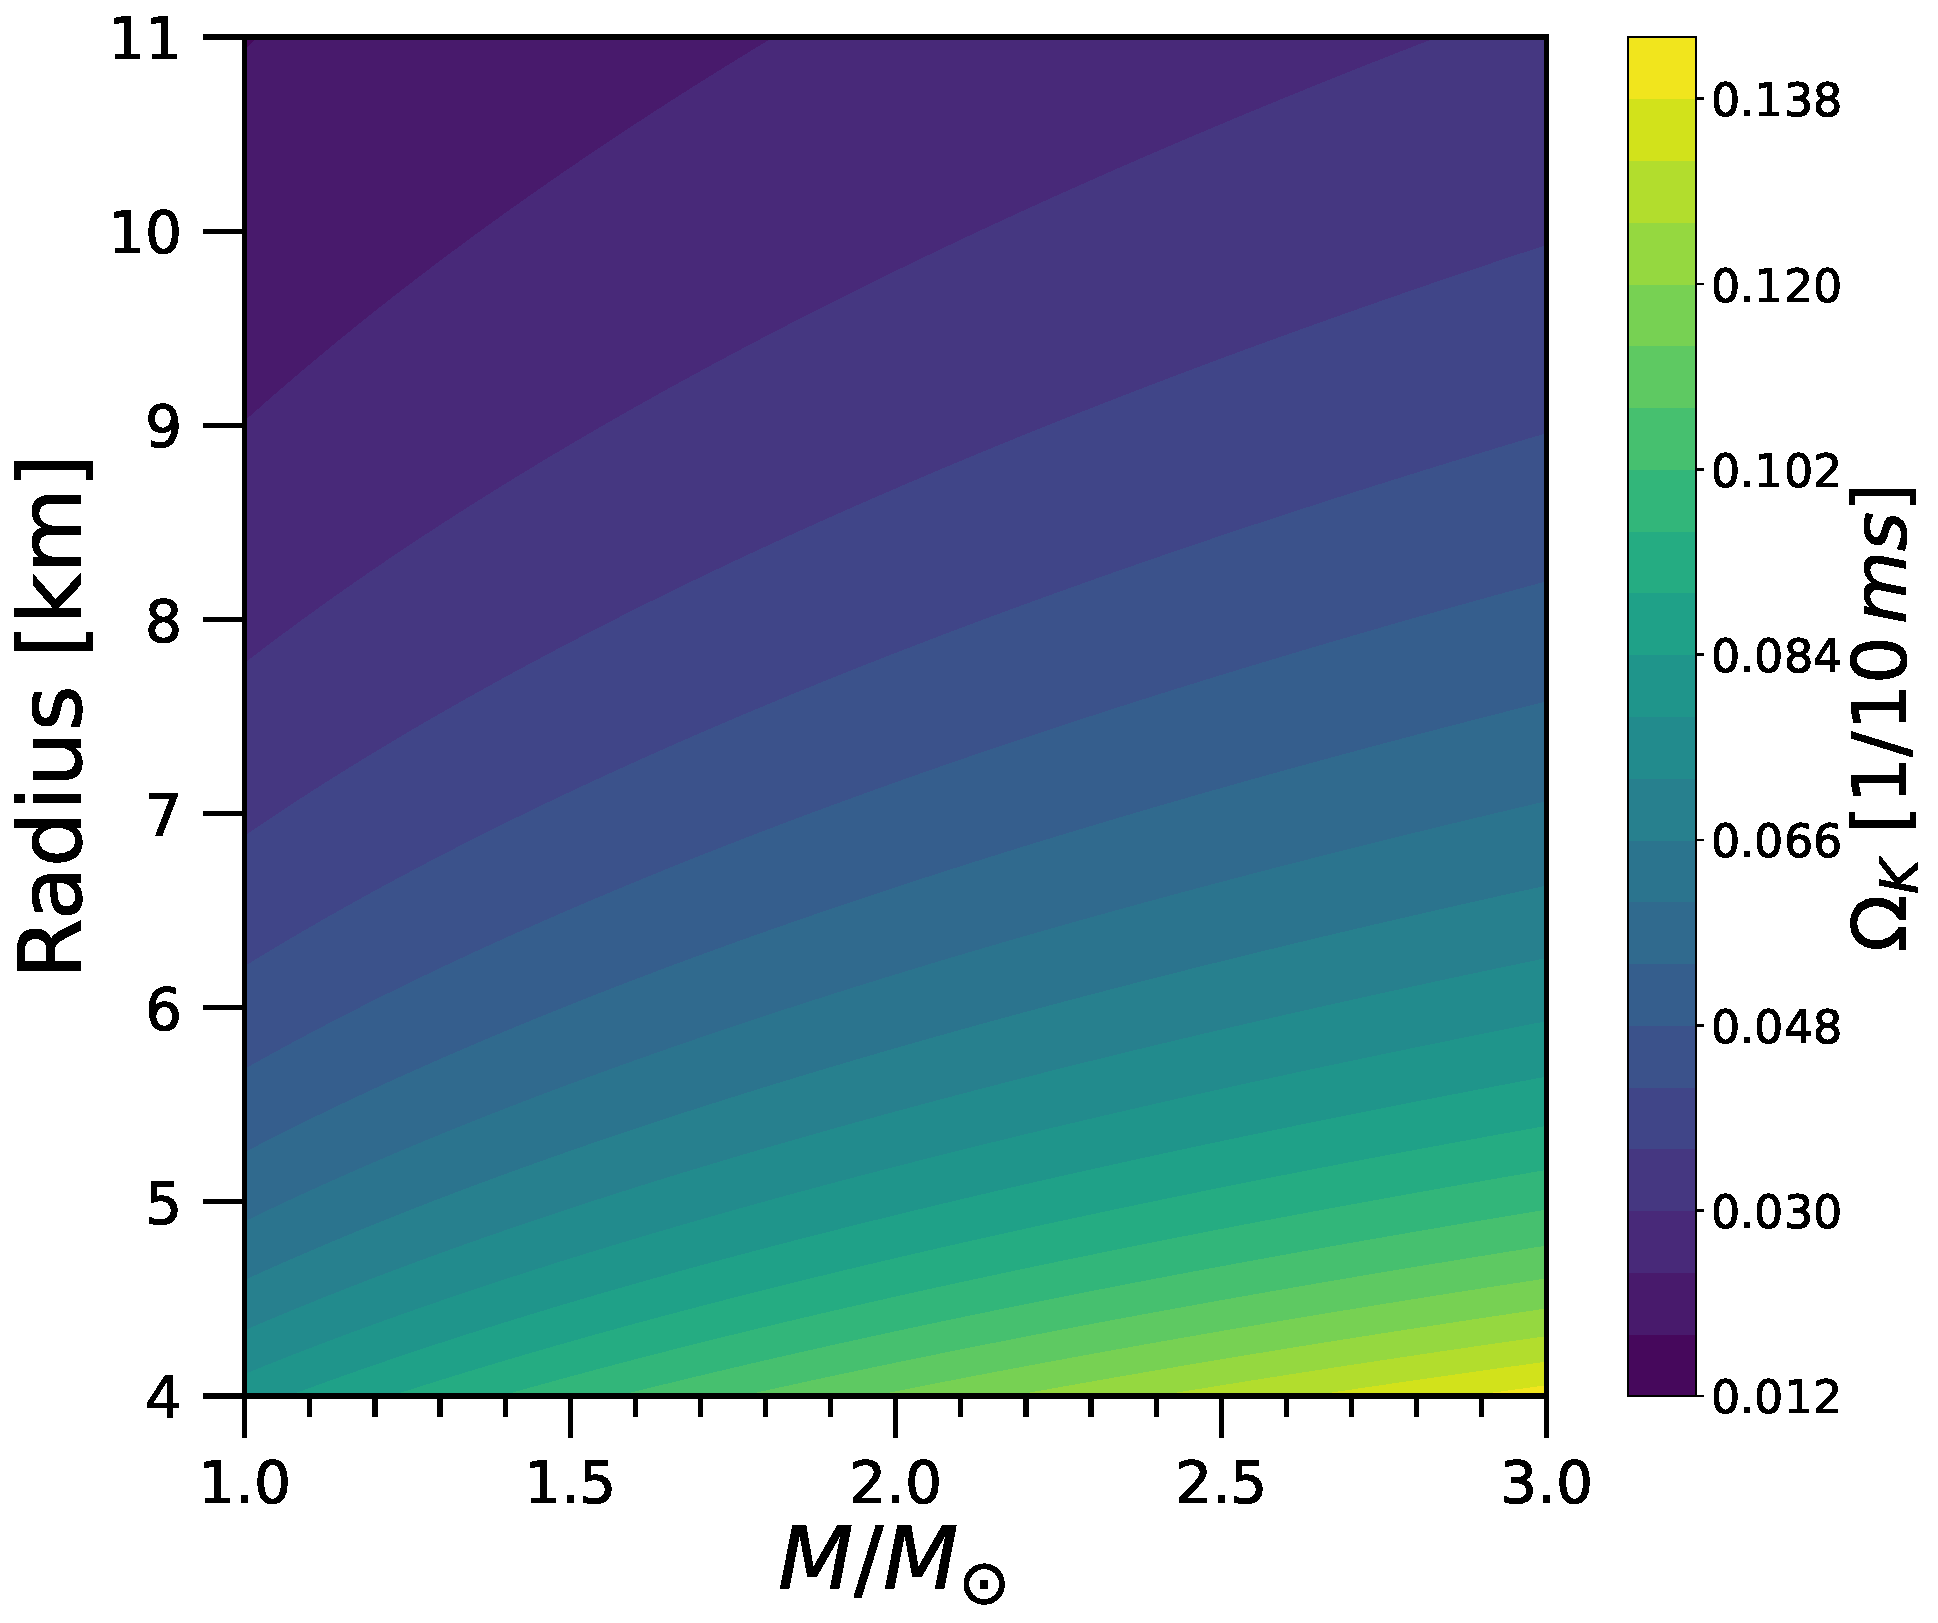
\includegraphics[width=0.95\linewidth]{./images/ns-m-radius-Omega_k.pdf}
		\captionof{figure}{Contour plot of the $\Omega_{K}$ Kerpler frequency calculated from the approximation in Eq. \eqref{eq:6}.}
	\end{figure}
\end{column}
\begin{column}{0.5\textwidth}
	\begin{figure}
		\centering
		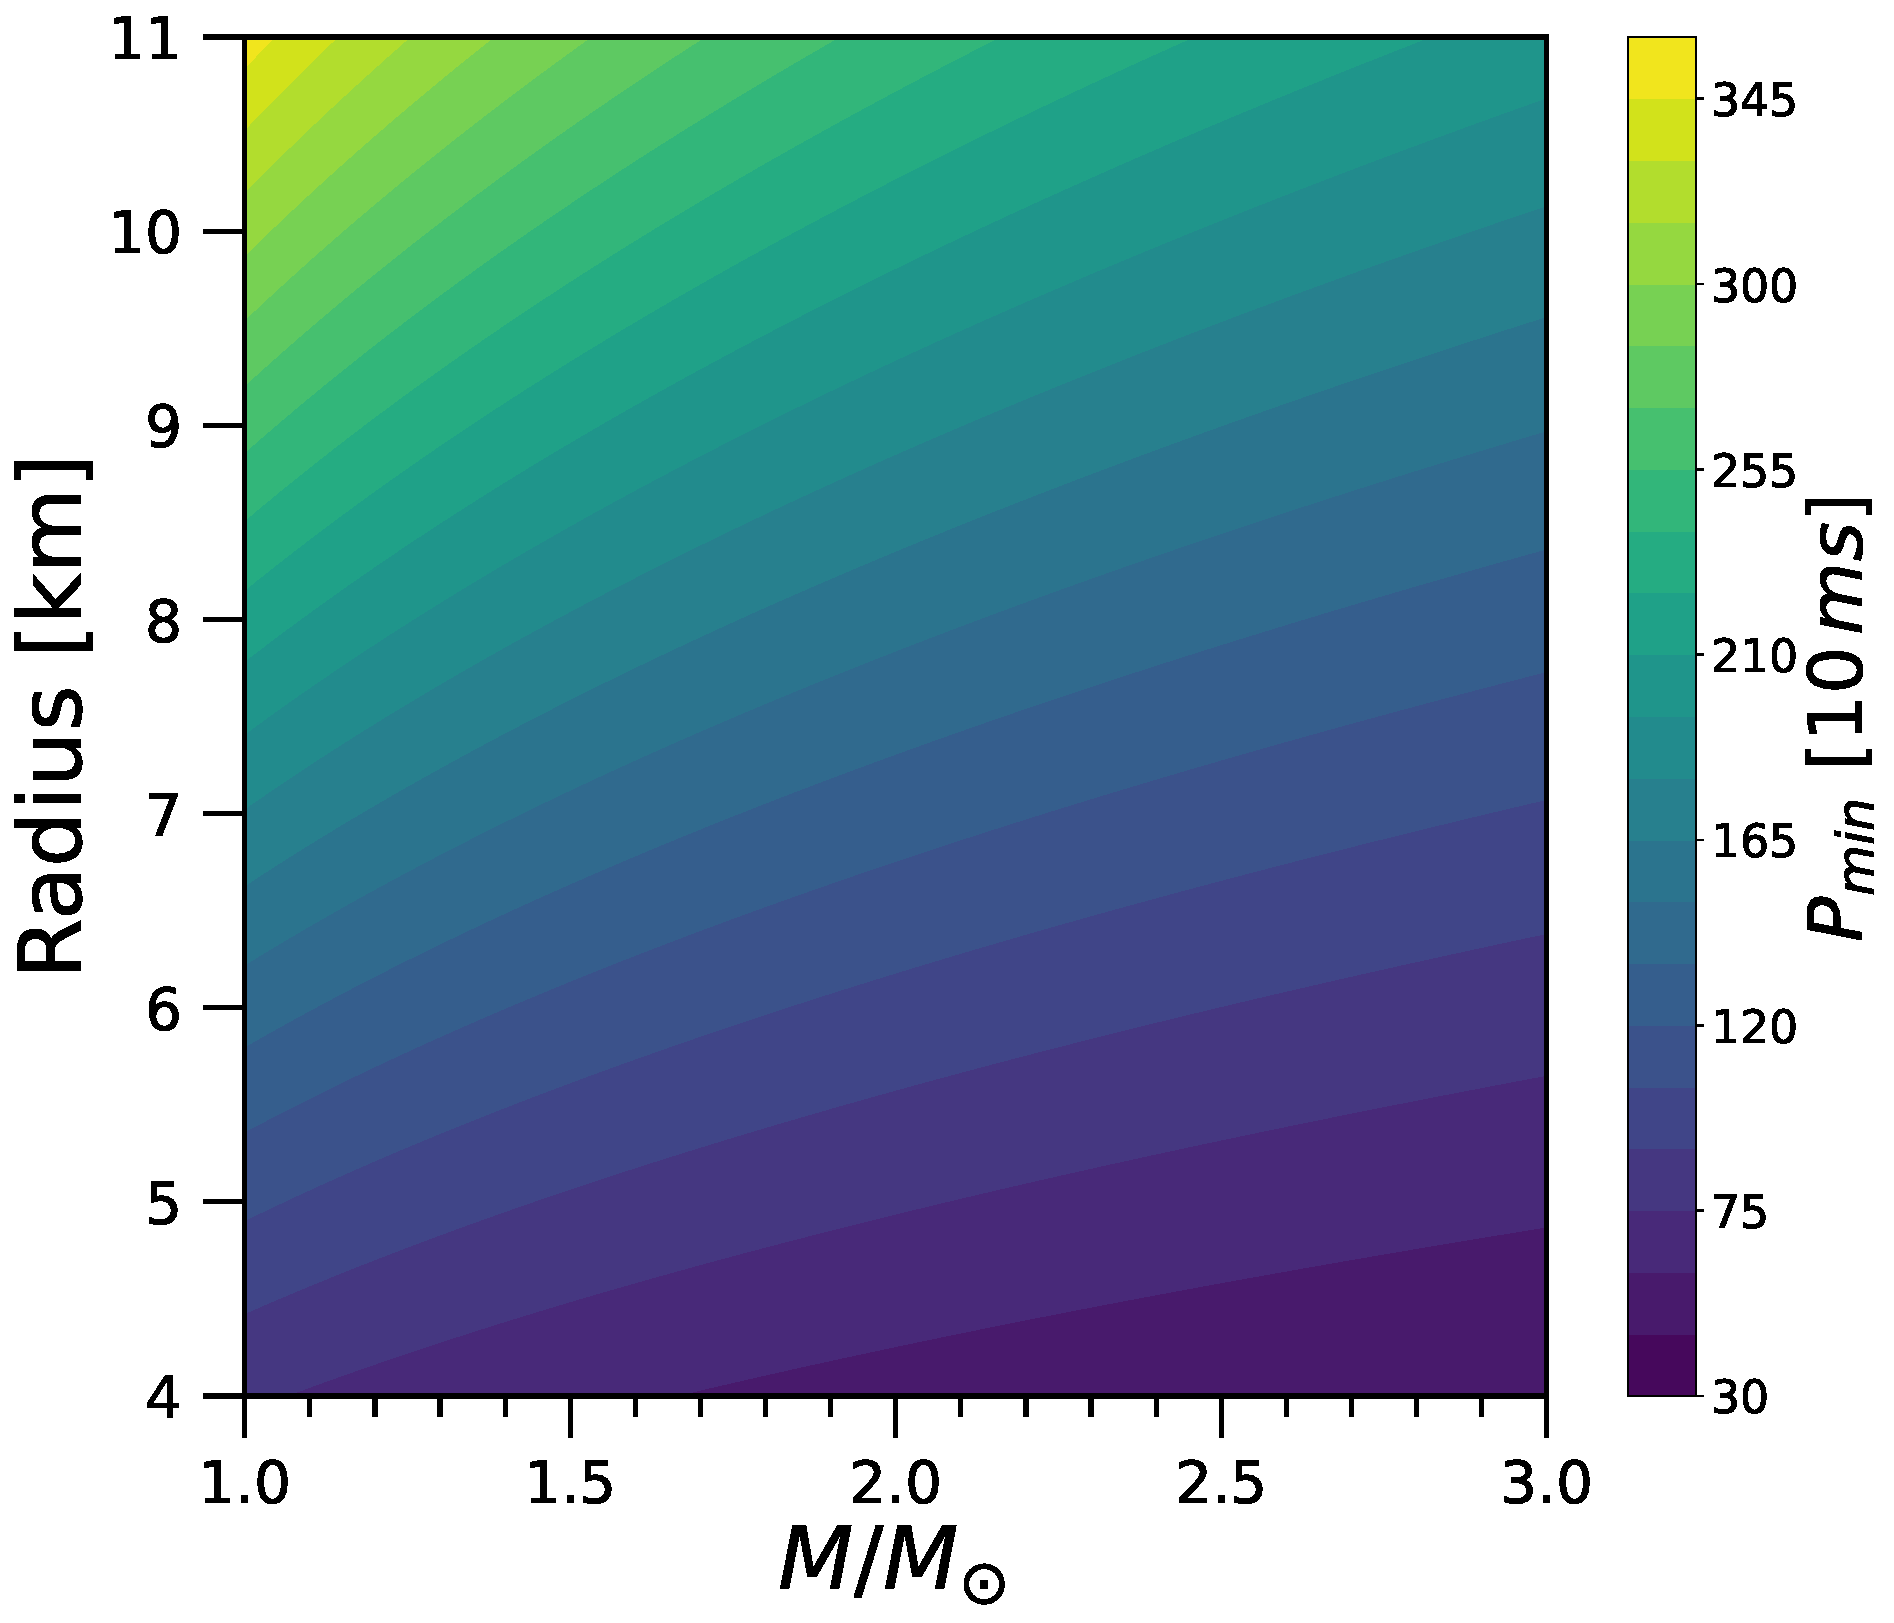
\includegraphics[width=0.95\linewidth]{./images/ns-m-radius-P.pdf}
		\captionof{figure}{Contour plot of the $P_{min}$ minimal rotation period calculated from the approximation in Eq. \eqref{eq:6}.}
	\end{figure}
\end{column}
\end{columns}

\end{frame}


